\documentclass{article}
\usepackage{graphicx} % Required for inserting images
\usepackage{hyperref}
\usepackage{amsmath}
\usepackage{longtable}
\usepackage{booktabs}
\title{PAT paper}
\author{Joseph Fish}

%\usepackage{biblatex}
\usepackage[backend=biber,
style=authoryear,
citestyle=authoryear]{biblatex} 
\addbibresource{latex/bibliograph.bib}


\date{March 2024}


\begin{document}

\section{Motivation}

Evictions in America are both remarkably common and remarkably concentrated. Each year, there are around 3.6 million eviction filings. These filings disproportionately occur within certain cities, within certain neighborhoods in those cities, and within certain buildings inside those neighborhoods. In the most extreme cases, like in Tuscon, Arizona, 300 buildings are responsible for over 66\% of eviction filings. In Philadelphia, only around 15\% of rental units will file an eviction in a given year, and about 10\% of all eviction filings come from just 2\% of units, and 25\% come from 10\% of all rental units. \\



\section{Empirical Setting}

The empirical setting for this project will be Philadelphia, Pennsylvania. Philadelphia is an ideal city for a number of reasons. On the demographic side, Philadelphia is the largest poor city in America, with a high eviction rate, high segregation, and a large Black population, making it a very useful case study for understanding America's low income housing market. On the data side, Philadelphia is unique in that it has a rental registry, meaning I can see exactly which properties are rental units in each year. Other studies have had to rely on owner occupancy exemptions to identify rental properties, which is problematic because it conflates rental units with Airbnbs and vacation homes. \\

Additionally, Philadelphia has very good historical eviction data, and, importantly, the eviction data contain contract rents, which let me see normally hard to observe rent prices for low income units. Finally, on the policy side, Philadelphia had a large change in their tenant protections in 2022, where they now make eviction cases go through mediation, leading to an approximately 30\% decline in eviction filings, relative to a pre-pandemic baseline.

\section{Stylized Facts about Philadelphia's Low Income Housing Market}

In this section, I lay out a series of motivating empirical facts about Philadelphia's low income housing market. Beginning with a map of Philadelphia (figure \ref{fig:philly-map}), I show that evictions in Philadelphia are geographically very concentrated in the predominately poor and highly segregated neighborhoods of West and North Philadelphia.


\begin{figure}[htbp]
    \centering
    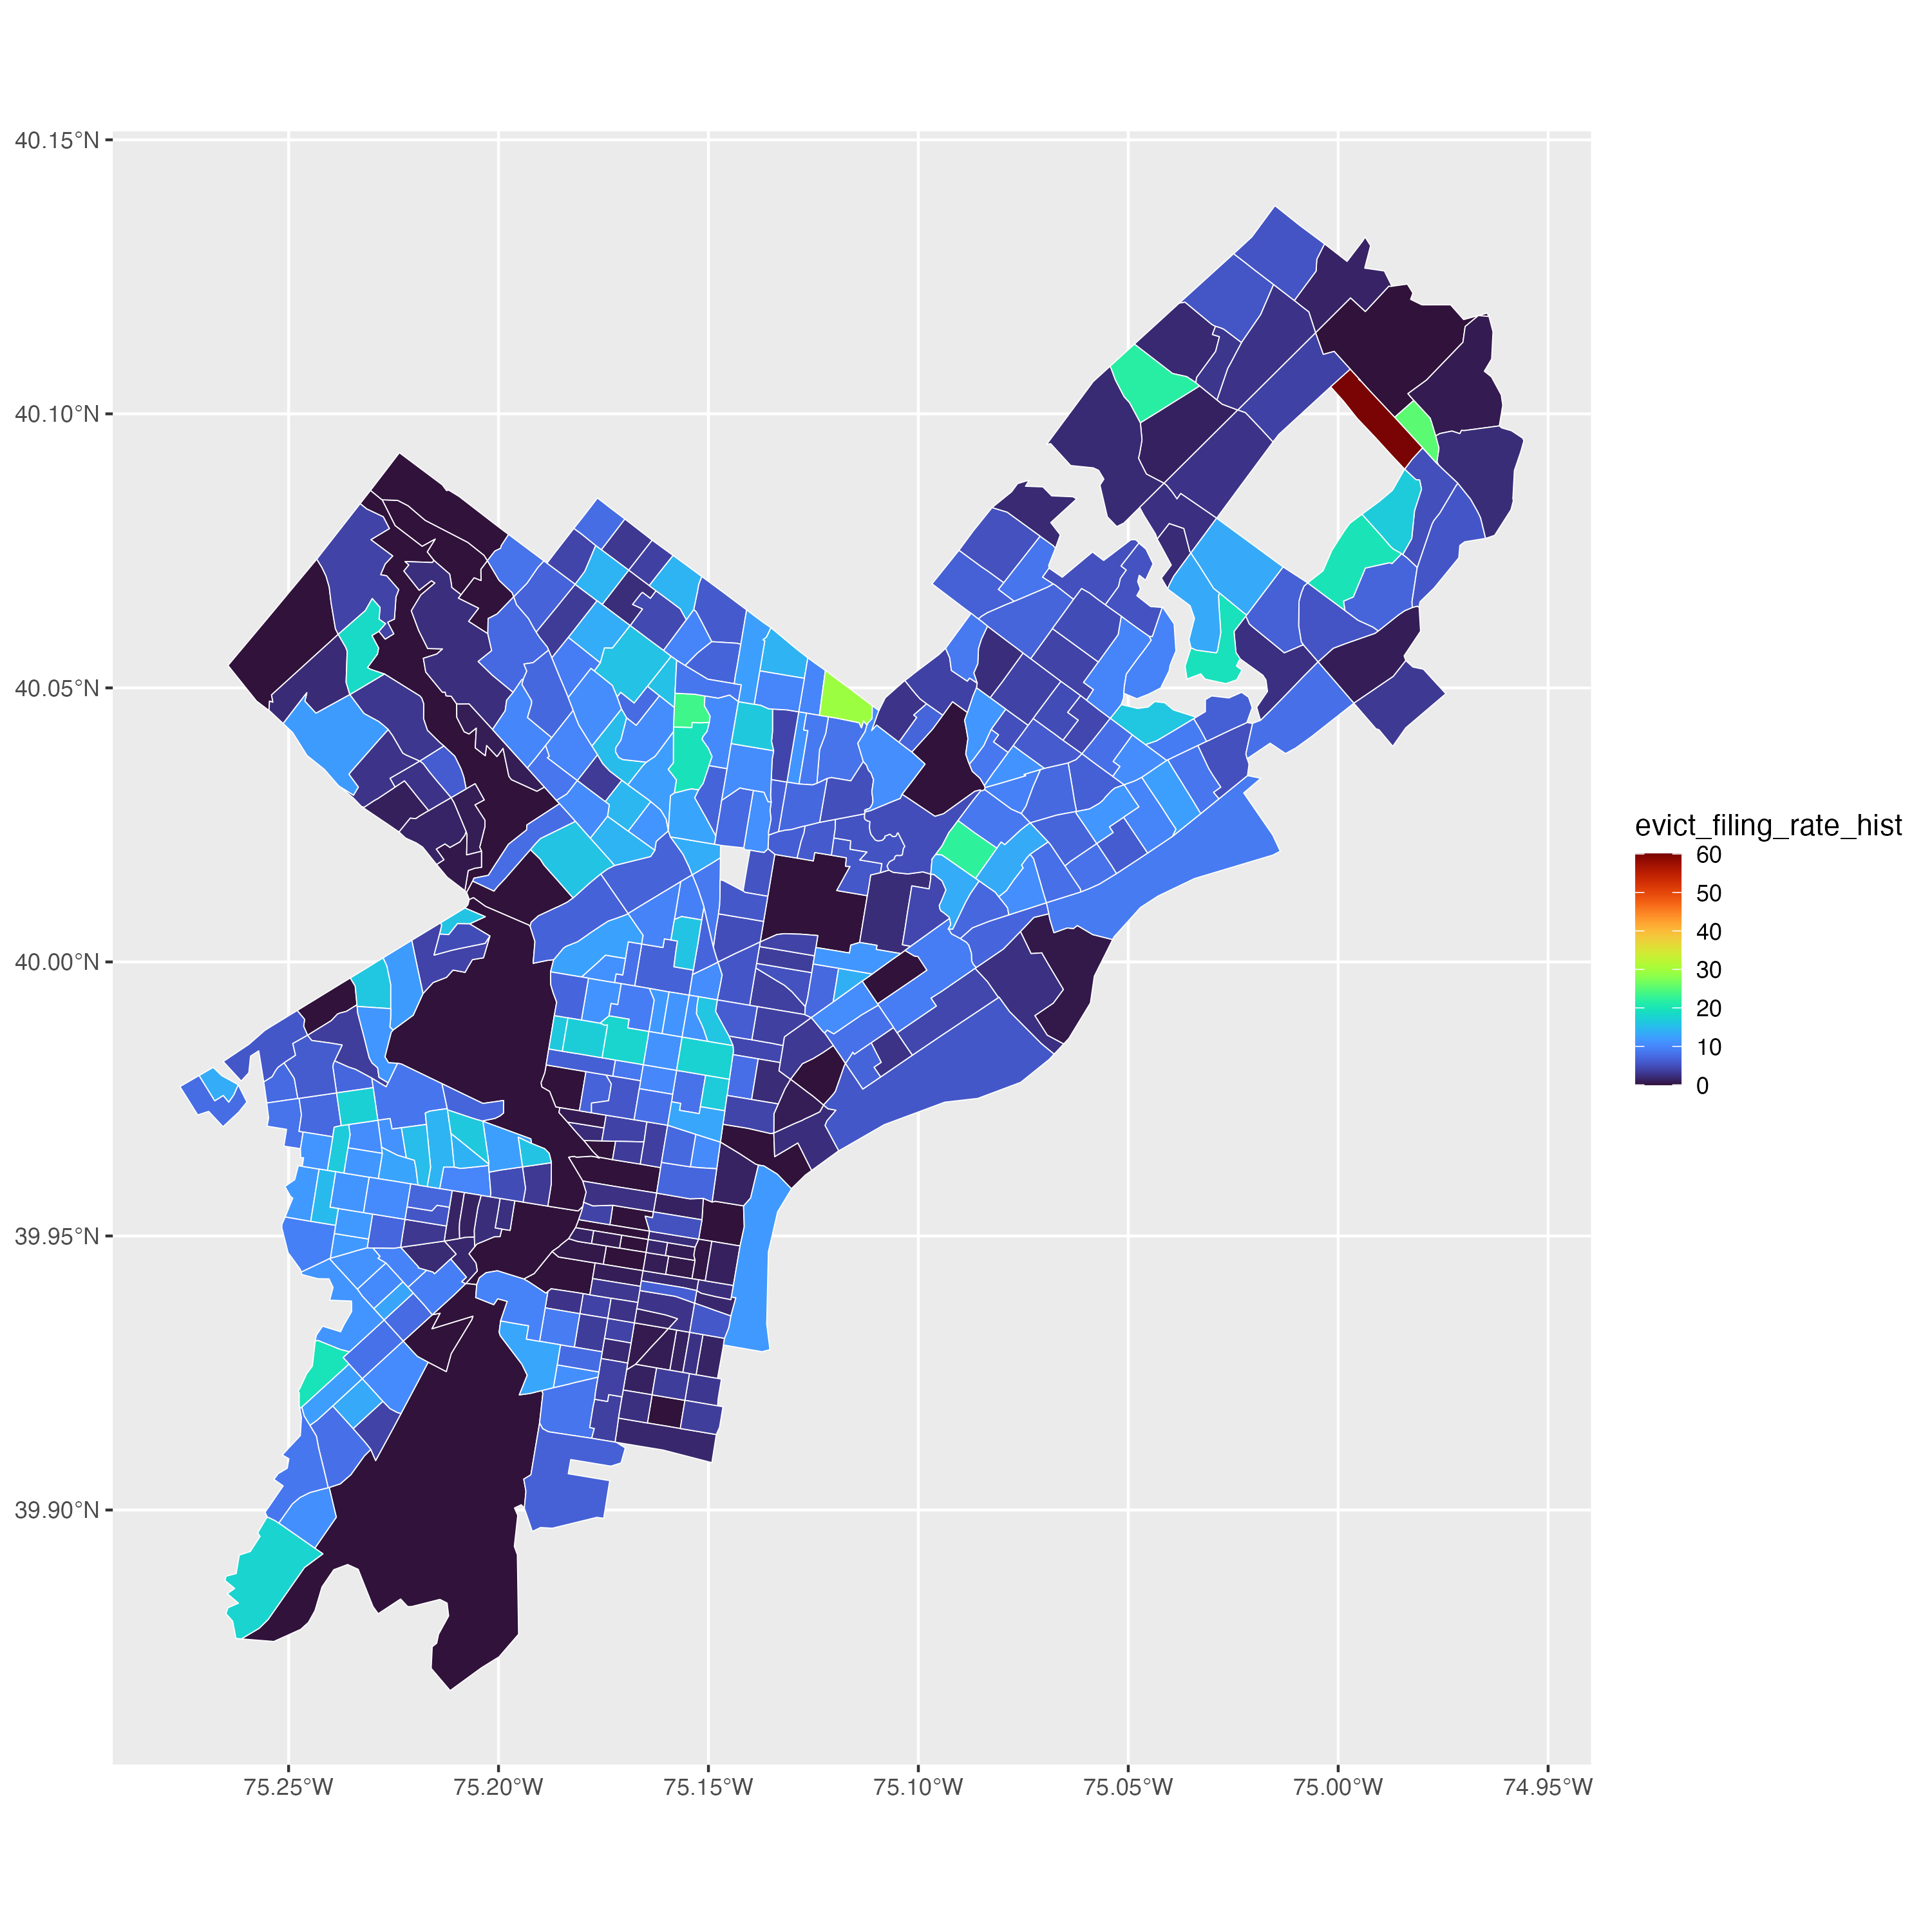
\includegraphics[width=1\linewidth]{figs/evict_filing_rate_hist.png}
    \caption{Evictions in Philadelphia (2019)}
    \label{fig:philly-map}
\end{figure}

Secondly, I show that, when looking across properties, evictions are concentrated in a handful of buildings. To show this, I merged the eviction data, which contain the defendant's address, with the rental registry and the parcel data in Philadelphia. This lets me know which properties are rental units in a given year, as well as the number of rental units that are in each property. Doing this allows me to plot the CDF of eviction filings alongside the CDF of rental units. \\

As figure \ref{fig:philly-evict-parcel} shows, the vast majority of rental units do not file an eviction in a typical year. Of the properties that do file an eviction, most file only one. Collectively, about 10\% of all eviction filings come from just 2\% of units. \\

\begin{figure}[htbp]
    \centering
    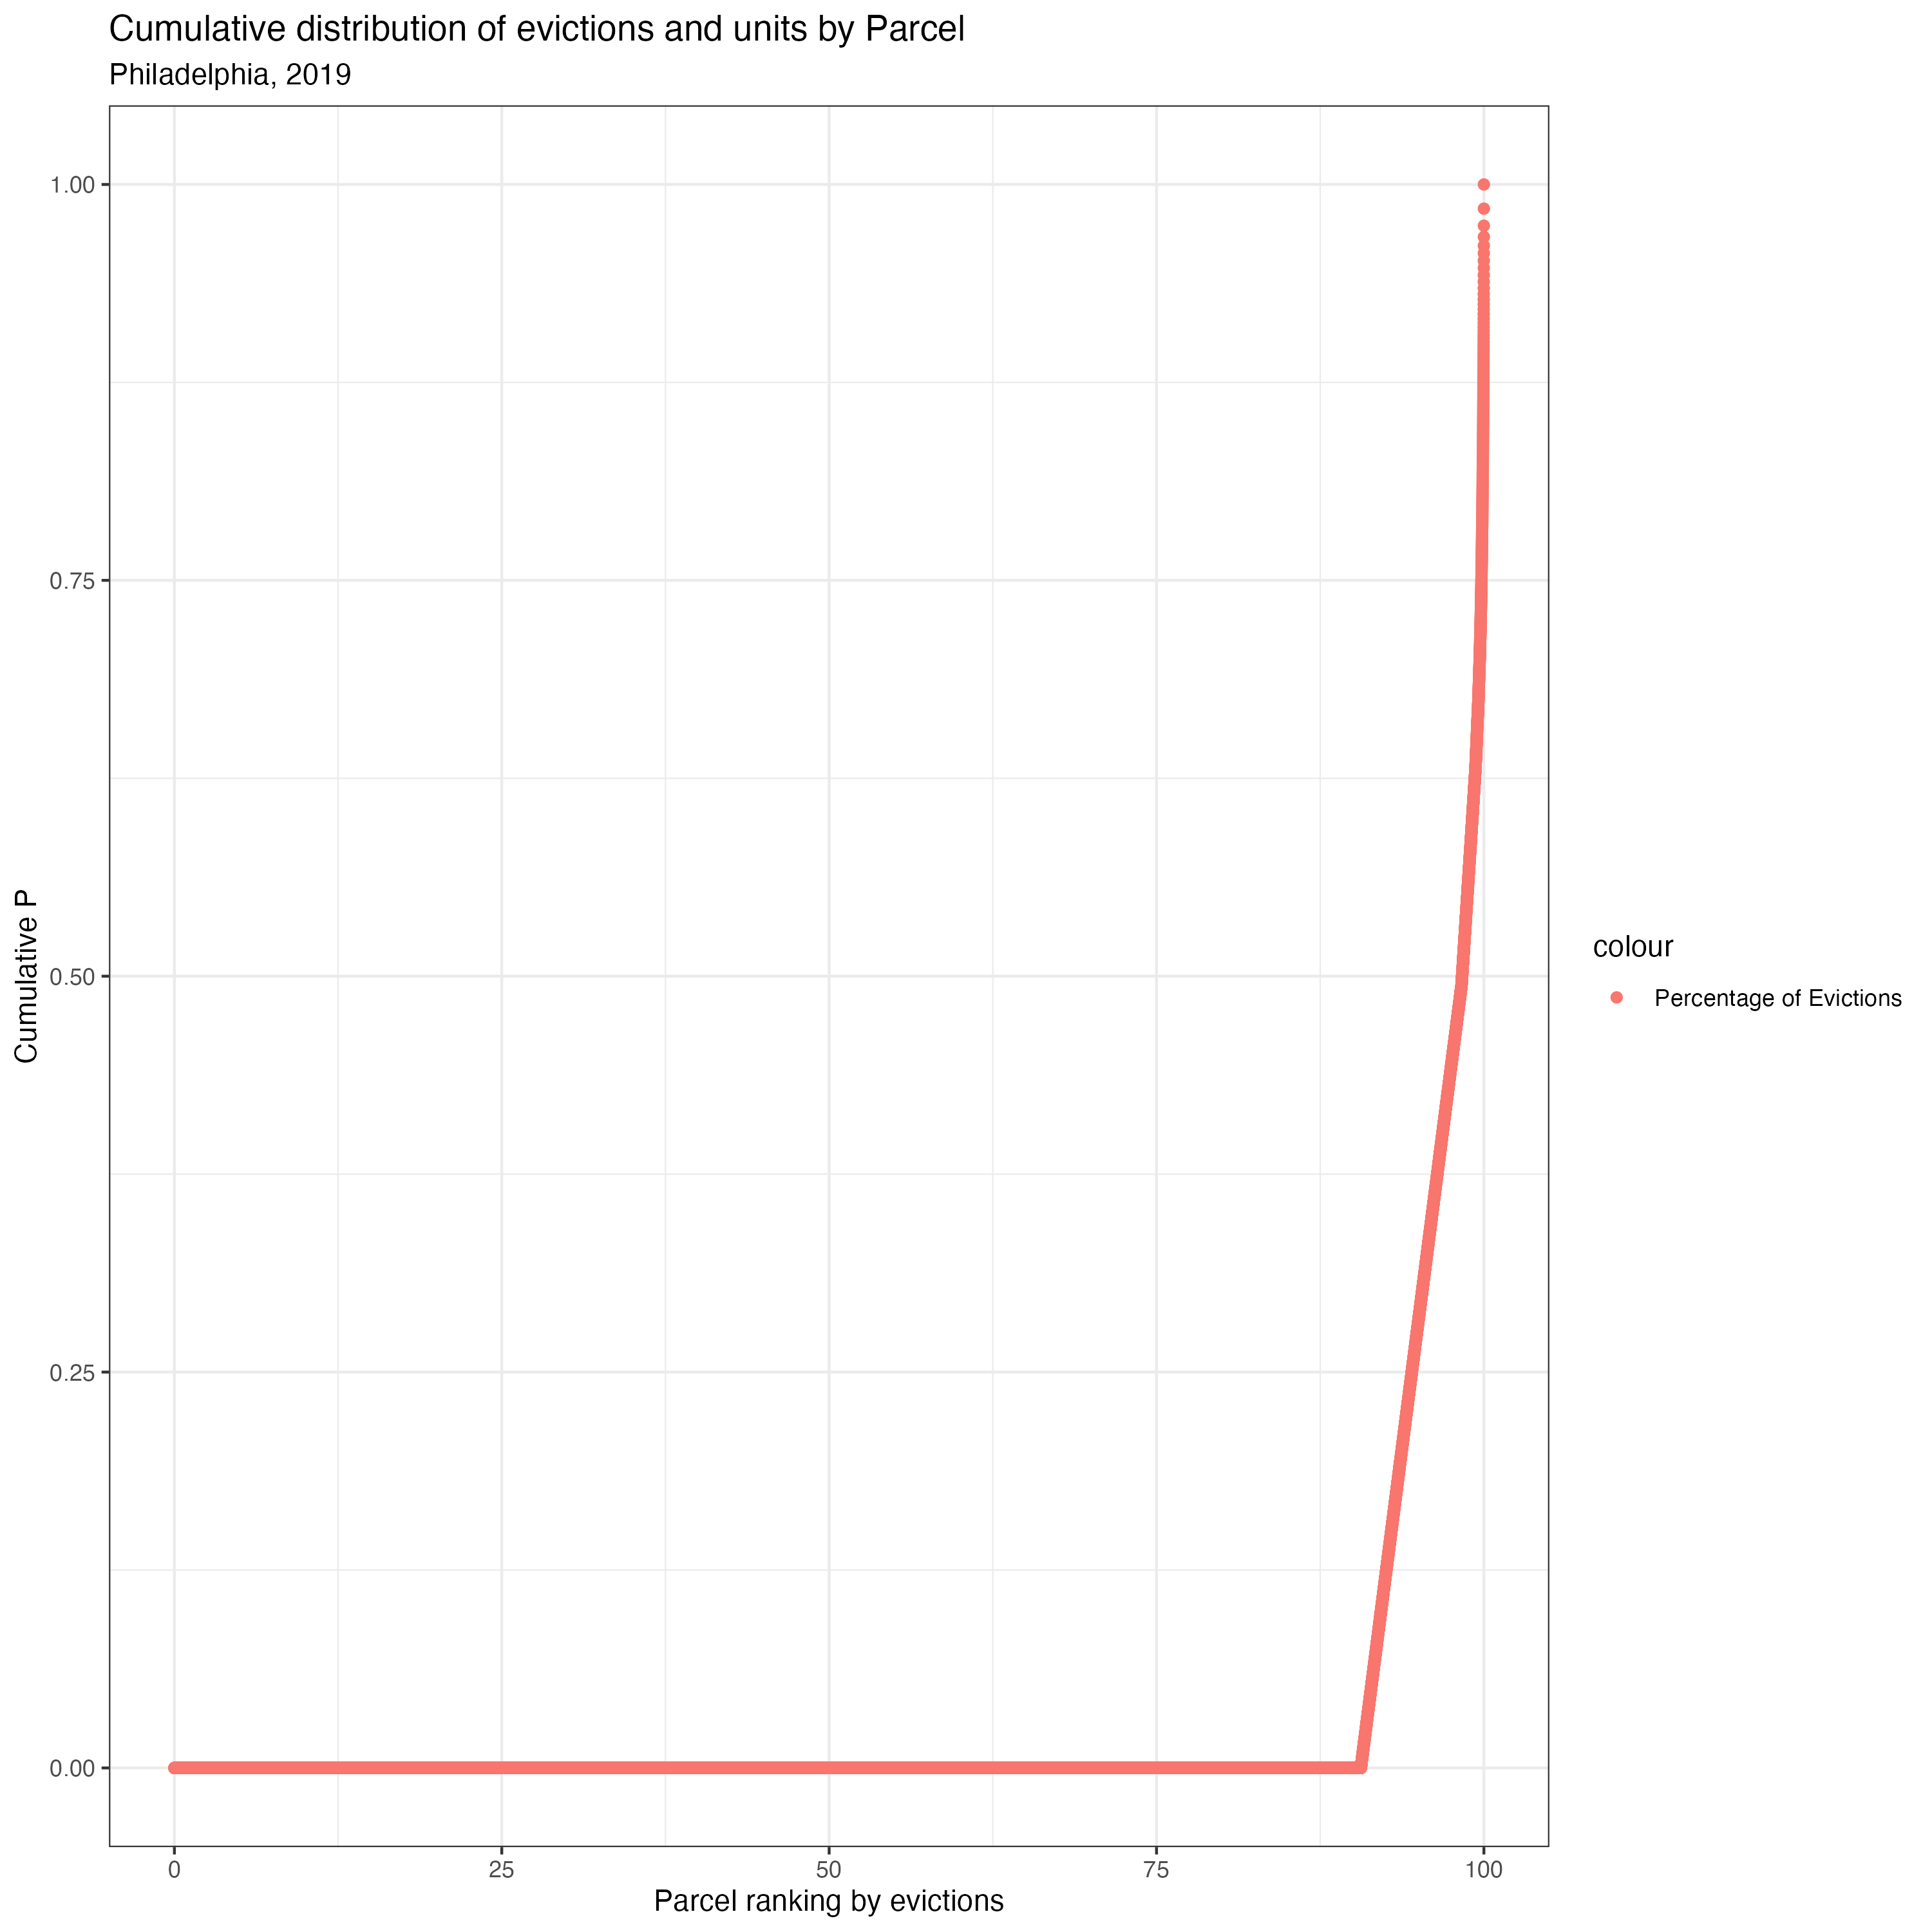
\includegraphics[width=1\linewidth]{figs/cumulative_evict_dist_parcels.png}
    \caption{Evictions in Philadelphia}
    \label{fig:philly-evict-parcel}
\end{figure}

Third, in table \ref{tab:philly-rent},I group eviction filings by whether they were filed by one of the top-100 evicting plaintiffs in each year. I show that there are not substantial differences in rent prices between filings by high / low evicting plaintiffs.\\

\begin{table}[htbp]
    \begin{longtable}{l|rrrr}
\caption*{
{\large Summary Statistics on Philadelphia Rent Prices} \\ 
{\small 2010-2019}
} \\ 
\toprule
\multicolumn{1}{l}{} & \multicolumn{2}{c}{Rent} & \multicolumn{2}{c}{Number of Evictions} \\ 
\cmidrule(lr){2-3} \cmidrule(lr){4-5}
\multicolumn{1}{l}{} & non-Top Evictor & Top Evictor & non-Top Evictor & Top Evictor \\ 
\midrule\addlinespace[2.5pt]
2010 & $675$ & $634$ & 14649 & 6674 \\ 
2011 & $685$ & $654$ & 14979 & 6498 \\ 
2012 & $700$ & $654$ & 15271 & 6642 \\ 
2013 & $700$ & $675$ & 15366 & 6064 \\ 
2014 & $725$ & $707$ & 15645 & 6257 \\ 
2015 & $750$ & $725$ & 14395 & 5891 \\ 
2016 & $750$ & $800$ & 14994 & 5622 \\ 
2017 & $775$ & $825$ & 14627 & 5748 \\ 
2018 & $800$ & $970$ & 11987 & 3735 \\ 
2019 & $850$ & $1,050$ & 11763 & 3473 \\ 
\bottomrule
\end{longtable}


    \caption{Philadelphia Rent}
    \label{tab:philly-rent}
\end{table}


Finally, in figure \ref{fig:philly-year}, I show that evictions declined substantially during COVID and have held at lower rates than the pre-pandemic baseline. \\

\begin{figure}[htbp]
    \centering
    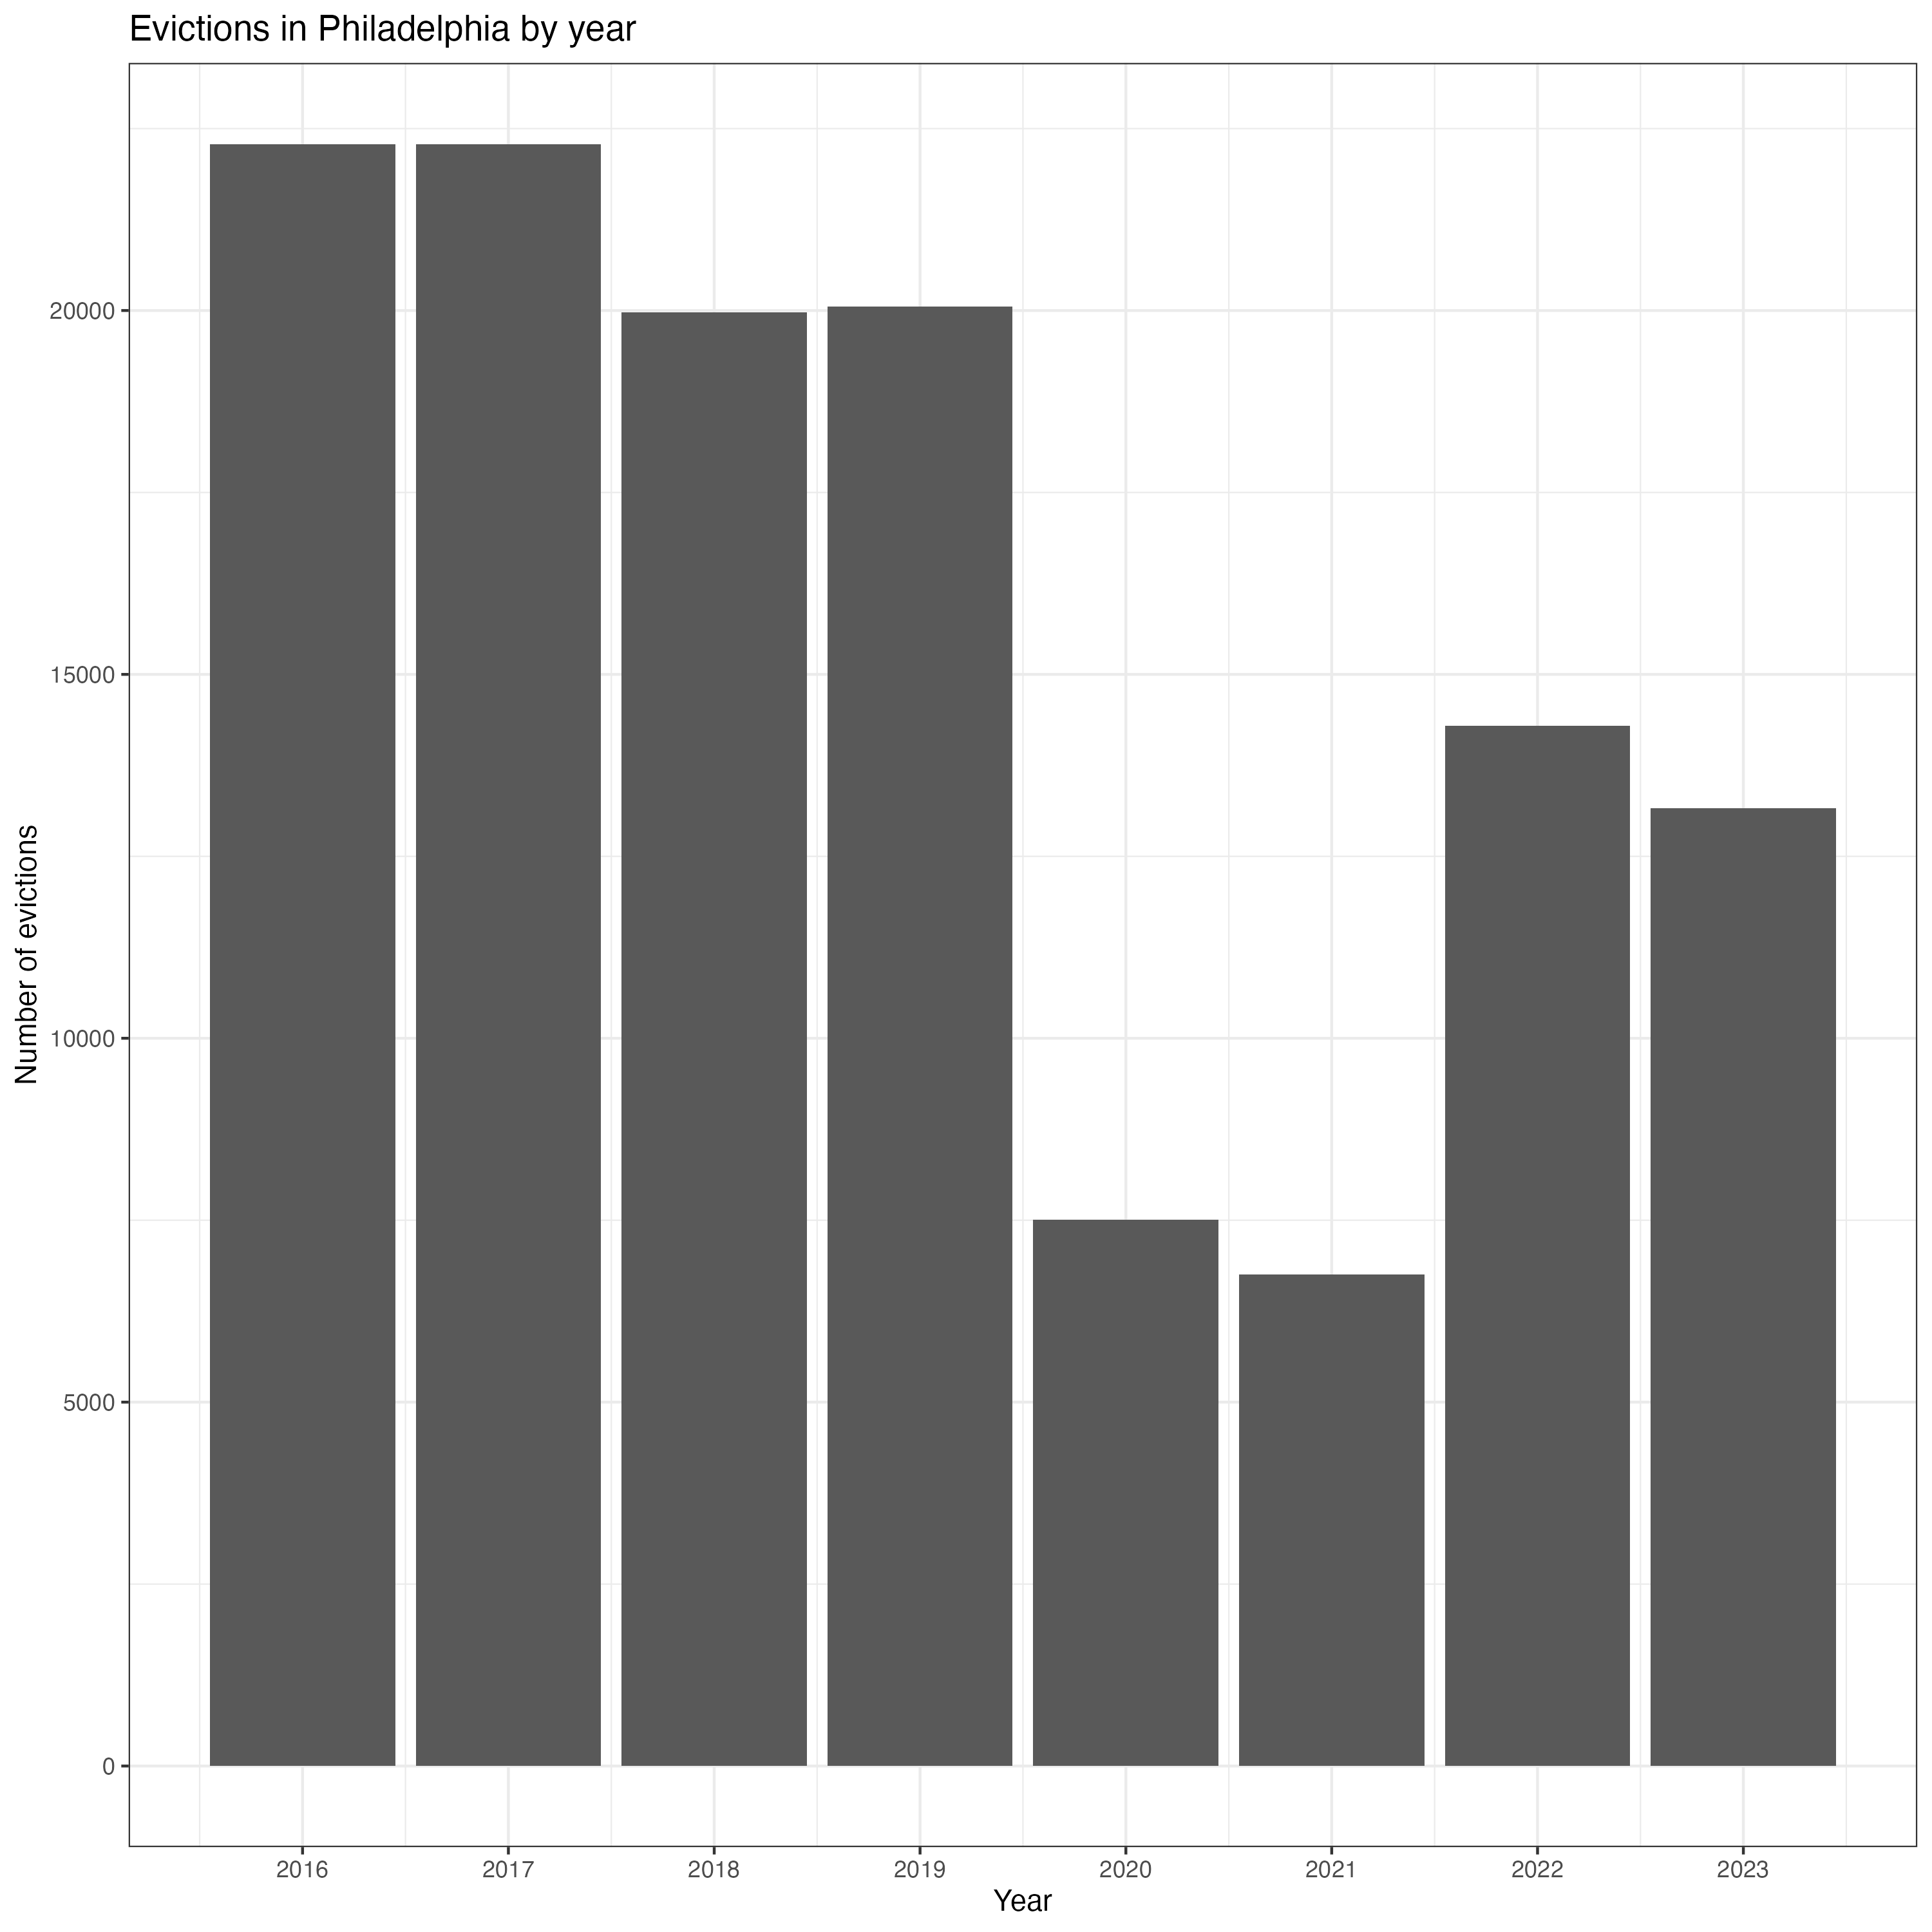
\includegraphics[width=1\linewidth]{figs/evict_by_year.png}
    \caption{Evictions in Philadelphia}
    \label{fig:philly-year}
\end{figure}

Taken together, these empirical facts show that there are interesting patterns of spatial clustering, patterns of landlord behavior, and possible policy variation I could exploit.
\pagebreak
\section{Research Questions and Empirical Specifications}

\subsection{Descriptive Evidence on Pricing and Eviction Filing Behavior}

\section{Overview of literature}
\subsection{Price Gradients in Rental Markets}
\begin{itemize}
    \item Desmond and Wilmers
    \item alpha in affordable housing
    \item early urban lit on Chicago / other segregated places
\end{itemize}

\subsection{New Econ stuff on Evictions}
\begin{itemize}
    \item Eviction is bad for tenants
    \item Eviction / landlord learning model
    \item Landlord responses to changes in tenant protections (more protections, landlord exit, higher prices)
\end{itemize}

\subsection{Recent IO literature on monopoly pricing}


\section{Overview of Data}

\subsection{Why rental markets are so hard}
\subsection{Why I can study rental markets}
\subsection{InfoUSA}
\subsection{Search Patterns}
- Chris timmons stuff on search; reference my mini lit review on search
\subsection{Property level vacancy rates...}
ways to try and compute them based on flows from infoUSA data... this will be empirically challenging, particularly for low income rental markets 

\subsection{A model of market power}
\paragraph{Is it all segregation and demand?}
\paragraph{Role of Search Costs}



\subsection{A model of landlord-tenant bargaining}
\subsection{A model of landlord exit}



\end{document}